% !TeX root = ../../Book1.tex
% 纲要标题：### 5.2 空间粘合与 van Kampen 定理
% 纲要位置：几何学计划纲要.md，第 284 行。
% 正文状态：初稿完成；尚未正式审核。

% 纲要内容开始
% 
% * 自由积及带关系群的最低准备
% * 细分道路和开覆盖的证明
% * 多重交集、基点选择与推广范围
% * 图、曲面和去点空间的群展示
% 
% 纲要内容结束

\section{空间粘合与 van Kampen 定理}
\label{g1:sec:0502}

圆周上的绕数记录绕行次数，但两个圆周在一点相接以后，仅记录各绕了几圈便不够了：先走左圈再走右圈，与先右后左未必能够互相变形。另一方面，若在这两个圆周上再粘一张圆盘，沿圆盘边界走出的某个词就会变成可以收缩的闭路。基本群因而同时记录“可以怎样走”和“哪些走法被填上的区域消去”。本节把这两件事分别写成生成元与关系，再证明它们确实由空间的开覆盖决定。

\subsection{自由积及带关系群的最低准备}
\label{g1:subsec:0502:01}

我们只补充当前计算所需的群论。群的单位元记为 \(1\)，群乘法的书写顺序沿用道路约定：\([\alpha][\beta]=[\alpha*\beta]\) 表示先走 \(\alpha\)，再走 \(\beta\)。一个词是有限个字母排成的序列；空词也允许，长度为零。

\begin{definition}[自由群]\label{g1:def:free-group}
	给定符号集合 \(S\)，对每个 \(s\in S\) 增加一个形式逆符号 \(s^{-1}\)。删去词中相邻的 \(ss^{-1}\) 或 \(s^{-1}s\)，直到不能再删，所得词称为约化词。所有约化词组成的\term[ziyouqun]{自由群}[free group]记为 \(F(S)\)：乘法是先连接两个词再约化，单位元为空词，逆元是倒转字母顺序并逐字取逆。若 \(S=\{a_1,\ldots,a_r\}\)，也记 \(F_r\)。
\end{definition}

这个定义需要排除约化顺序带来的歧义。每次删除都使长度下降。若两次可作的删除位置不交，先后次序可交换；若位置相交，局部词只能是 \(ss^{-1}s\) 或 \(s^{-1}ss^{-1}\)，两种删除得到同一个单字母。对词长归纳：任意两条约化过程的第一步或者相同，或者经过上述交换抵达同一较短词，再用归纳假设，最终约化词一致。因此连接后约化是良定义的，而且把三个词一起连接时，无论先约化哪一段，最后结果相同，这就证明了结合律。逆元公式通过逐对消去验证。

任意指定一族元素 \(h_s\in H\)，其中 \(H\) 为群，都恰好确定一个同态 \(F(S)\to H\)：将 \(s\) 替换为 \(h_s\)，将 \(s^{-1}\) 替换为 \(h_s^{-1}\)，再按顺序相乘。删除相邻逆字母不改变乘积，故映射良定义；同态性来自连接词，唯一性来自每个词都由这些字母组成。这就是“自由”的精确含义：除群公理迫使成立的等式外，没有另加关系。特别地，\(F(\{a\})\cong\mathbb Z\)，而在 \(F(\{a,b\})\) 中，\(ab\) 与 \(ba\) 是不同的约化词。

空间的不同部分往往已经有各自的基本群，我们希望先保留每部分原有的关系，再把它们放在一起，而不提前要求不同部分的元素交换。

\begin{definition}[自由积]\label{g1:def:free-product}
	设 \((G_\alpha)_{\alpha\in A}\) 为一族群。它们的\term[ziyouji]{自由积}[free product] \(\mathop{*}_{\alpha\in A}G_\alpha\) 由下列约化词组成：每个字母是某个 \(G_\alpha\) 的非单位元，相邻字母来自不同的群。乘法是连接词，再把同一群中相邻的两个字母按该群的乘法合并，并删去出现的单位元。不同群中的字母保留所属群的标签。
\end{definition}

约化的唯一性可用与自由群相同的长度归纳证明。两处不相交的合并可以交换；相交时涉及同一群中的三个连续元素，两种合并最终一致正是该群的结合律，乘积为单位元时继续删除即可。因此这确实给出一个群，每个 \(G_\alpha\) 通过单字母词嵌入其中。对任一群 \(H\) 及同态 \(f_\alpha:G_\alpha\to H\)，公式
\[
	f(g_1\cdots g_m)=f_{\alpha_1}(g_1)\cdots f_{\alpha_m}(g_m)
\]
与约化相容，给出唯一的同态 \(f:\mathop{*}_\alpha G_\alpha\to H\)。两群情形的泛性质写成下图，其中两条斜箭头是给定的同态，虚线箭头是唯一延拓：
\[
	\begin{tikzcd}[column sep=large]
		G \arrow[r,"j_G"] \arrow[dr,"f_G"'] & G*H \arrow[d,dashed,"f"] & H \arrow[l,"j_H"'] \arrow[dl,"f_H"]\\
		& K &
	\end{tikzcd}
\]
例如 \(\mathbb Z*\mathbb Z=F_2\)，与直积 \(\mathbb Z\times\mathbb Z\) 不同：直积中两坐标的元素交换，自由积中一般不交换。

接着说明怎样加入关系。子群 \(N\subseteq G\) 称为\term[zhengguiziqun]{正规子群}[normal subgroup]，若对所有 \(g\in G\) 有 \(gNg^{-1}=N\)。这个条件保证陪集乘法 \((gN)(hN)=ghN\) 不依赖代表，从而定义\term[shangqun]{商群}[quotient group] \(G/N\)。给定 \(R\subseteq G\)，要使每个 \(r\in R\) 都成为单位元，必须同时消去它们的逆、乘积和所有共轭。因此包含 \(R\) 的最小正规子群为
\[
	\langle\!\langle R\rangle\!\rangle
	=\left\{\prod_{j=1}^{m}g_jr_j^{\varepsilon_j}g_j^{-1}:
	m\ge0,\ r_j\in R,\ \varepsilon_j=\pm1,\ g_j\in G\right\}.
\]
右边对乘法、逆及共轭封闭，且任何包含 \(R\) 的正规子群都包含右边，因而确实具有所说的最小性。它称为 \(R\) 的\term[zhengguibibao]{正规闭包}[normal closure]。

\begin{definition}[群展示]\label{g1:def:group-presentation}
	若 \(R\) 是自由群 \(F(S)\) 中的一组词，则
	\[
		\langle S\mid R\rangle=F(S)/\langle\!\langle R\rangle\!\rangle
	\]
	称为由生成元 \(S\) 和关系词 \(R\) 给出的\term[qunzhanshi]{群展示}[group presentation]。写关系 \(u=v\) 等价于把 \(uv^{-1}\) 加入关系词。
\end{definition}

由最小性可知，一个映射 \(S\to H\) 恰好在所有关系词映成 \(1\) 时延拓为 \(\langle S\mid R\rangle\to H\) 的同态。这个判据比“按关系化简到某种样子”更可靠，因为一般的群展示未必提供容易执行的唯一约化算法。例如
\[
	\langle a\mid a^m=1\rangle\cong\mathbb Z/m\mathbb Z\quad(m\ge1),\qquad
	\langle a,b\mid aba^{-1}b^{-1}=1\rangle\cong\mathbb Z^2.
\]
第二个同构可以直接验证：关系使 \(a,b\) 交换，所以每个词都能写成 \(a^pb^q\)；映射 \(a\mapsto(1,0)\)、\(b\mapsto(0,1)\) 给出同态到 \(\mathbb Z^2\)，并证明不同的整数对不会再被识别。这里既证明了这些表达能够覆盖所有元素，也证明了没有额外关系。

\subsection{细分道路和开覆盖的证明}
\label{g1:subsec:0502:02}

设 \(X=U\cup V\)。一条闭路未必全部落在 \(U\) 或 \(V\) 中，但紧参数区间可以切成有限段，每段落在其中一个开集。切出的段一般不是闭路；我们必须从公共基点走到各分点，再沿原路段前进，最后返回基点。不同接回方式之间的差别恰好发生在交集内，这便说明为什么群的关系应来自 \(U\cap V\)。

\begin{theorem}[van Kampen 定理]\label{g1:thm:van-kampen}
	设拓扑空间 \(X=U\cup V\)，其中 \(U,V\) 都开且道路连通，\(U\cap V\) 也道路连通，并取 \(x_0\in U\cap V\)。记包含映射诱导的同态为
	\[
		i_U:\pi_1(U\cap V,x_0)\to\pi_1(U,x_0),\qquad
		i_V:\pi_1(U\cap V,x_0)\to\pi_1(V,x_0).
	\]
	则两包含映射诱导满同态
	\[
		\Phi:\pi_1(U,x_0)*\pi_1(V,x_0)\longrightarrow\pi_1(X,x_0),
	\]
	其核恰为所有 \(i_U(\omega)i_V(\omega)^{-1}\) 的正规闭包。因此
	\begin{equation}\label{g1:eq:van-kampen-quotient}
		\pi_1(X,x_0)\cong
		\frac{\pi_1(U,x_0)*\pi_1(V,x_0)}
		{\langle\!\langle i_U(\omega)i_V(\omega)^{-1}:\omega\in\pi_1(U\cap V,x_0)\rangle\!\rangle}.
	\end{equation}
\end{theorem}

这就是\term[vankampendingli]{van Kampen 定理}[van Kampen theorem]。\footnote{Egbert Rudolf van Kampen（埃格伯特·鲁道夫·范坎彭，1908--1942），生于比利时，在荷兰求学，后在美国任教，研究拓扑与拓扑群。} 其中的关系只要求把交集中的同一条闭路在两边识别，并不声称 \(i_U,i_V\) 单射。例如交集中的圆圈可能已经在 \(U\) 内围成一个圆盘，此时它在 \(V\) 中的像也会被关系消去。式\eqref{g1:eq:van-kampen-quotient}有时称为沿交集群的合并自由积，但计算时仍应保留两条具体同态。

\begin{proof}
	记式\eqref{g1:eq:van-kampen-quotient}右边的群为 \(P\)，两因子到 \(P\) 的同态为 \(j_U,j_V\)。交集中的同一闭路在 \(X\) 中当然给出同一元素，故 \(\Phi\) 下降为同态 \(\bar\Phi:P\to\pi_1(X,x_0)\)。我们将对闭路构造反向映射，并逐一说明分段、连接道路和同伦都不会改变结果。

	先取闭路 \(\gamma:[0,1]\to X\)。开覆盖 \(\{\gamma^{-1}(U),\gamma^{-1}(V)\}\) 由\cref{g1:lem:lebesgue-number}有 Lebesgue 数，所以存在分点 \(0=t_0<\cdots<t_m=1\)，使每段 \(\gamma_k=\gamma|_{[t_{k-1},t_k]}\) 的像落在一个标记开集 \(A_k\in\{U,V\}\) 中；各段均线性重新参数化为 \([0,1]\)。在分点 \(y_k=\gamma(t_k)\) 处选道路 \(c_k:x_0\to y_k\)：若相邻标记不同，在 \(U\cap V\) 中选择；若相同，在该标记开集中选择。取 \(c_0,c_m\) 为常值道路。道路连通的假设保证这些选择存在。令
	\[
		W(\gamma)=\prod_{k=1}^{m}j_{A_k}\bigl([c_{k-1}*\gamma_k*\bar c_k]\bigr)\in P.
	\]
	每个括号内都是 \(A_k\) 中以 \(x_0\) 为基点的闭路。把它们在 \(X\) 中连接，连续出现的 \(\bar c_k*c_k\) 可相对端点缩去，因此 \(\bar\Phi(W(\gamma))=[\gamma]\)。

	若将 \(c_k\) 改为另一条允许的 \(d_k\)，记 \(h_k=[c_k*\bar d_k]\)。在相邻标记相同时，\(h_k\) 属于同一个因子；标记不同时，两条连接道路都在交集中，故 \(h_k\) 在两个因子中的像由 \(P\) 的关系识别。替换后第 \(k\) 项变为
	\[
		h_{k-1}^{-1}\,j_{A_k}([c_{k-1}*\gamma_k*\bar c_k])\,h_k,
	\]
	这里将 \(h_k\) 也记作其在 \(P\) 中的像。相邻的 \(h_kh_k^{-1}\) 依次消去，且 \(h_0=h_m=1\)，故 \(W(\gamma)\) 不变。

	在一段内部增加分点时，只需在同一个标记开集中增加一条连接道路；插入的反路与正路相消，所以值仍不变。如果某一段同时位于 \(U,V\)，要改变它的标记，可以先把两端连接道路都改选在 \(U\cap V\) 中。这在原标记和新标记下都允许，且刚刚已证明不影响乘积；随后该段对应的闭路全在交集中，换标记正是 \(P\) 中的一条关系。任意两种分段都有共同细分，细分后的标记可逐段改变。因此 \(W(\gamma)\) 不依赖这些选择。

	还须证明相对端点同伦不改变 \(W\)。设 \(H:[0,1]^2\to X\) 是 \(\gamma_0\) 到 \(\gamma_1\) 的同伦，且 \(H(0,t)=H(1,t)=x_0\)。对方形上的拉回开覆盖应用 Lebesgue 数引理，取足够细的矩形网格，使每个闭小矩形的像全在 \(U\) 或 \(V\) 中，并给它相应的标记。对每个网格顶点 \(v\)，选道路 \(c_v:x_0\to H(v)\)：若相邻小矩形出现两种标记，就在交集中选；否则在唯一的标记开集中选。左右边界顶点的 \(c_v\) 都取常值。对从顶点 \(v\) 到 \(w\) 的有向网格边 \(e\)，记
	\[
		E(e)=j_A([c_v*(H|_e)*\bar c_w])\in P,
	\]
	其中 \(A\) 是任一相邻小矩形的标记。若有两种标记，该闭路全在交集中，故两种取法给出同一元素；反向边的元素为 \(E(e)^{-1}\)。

	对任一小矩形，把下边、右边、上边、左边分别按向右、向上、向右、向上定向，得到元素 \(b,r,t,\ell\)。将矩形边界沿矩形内的直线缩到左下角，再复合 \(H\)，便给出该标记开集内保持基点的收缩；其基点通过 \(c_v\) 接到 \(x_0\) 不改变可收缩性。消去中间连接道路便得
	\[
		brt^{-1}\ell^{-1}=1,\qquad\text{即 }br=\ell t.
	\]
	这条等式允许把网格路径的“下边后右边”换成“左边后上边”。逐格从最下一行向上移动：同一行中相邻矩形的公共竖边一正一反，替换时相消；扫完整行后，下面的水平边乘积换成上面的水平边乘积，外侧只留下左右边界的竖边。后者经 \(H\) 都是常值，元素为 \(1\)。逐行应用，得到整个方形底边与顶边的乘积相等，即 \(W(\gamma_0)=W(\gamma_1)\)。\cref{g1:fig:van-kampen-grid}显示的正是这个局部替换，而非交换不相邻的群元素。

	因此 \(W\) 给出映射 \(\Psi:\pi_1(X,x_0)\to P\)。连接两条闭路时，把两套分段接在一起，并在接合处取常值连接道路，就有 \(W(\alpha*\beta)=W(\alpha)W(\beta)\)，故 \(\Psi\) 为同态。已经证明 \(\bar\Phi\Psi\) 恒等。若闭路全在 \(U\) 中，取只有一段的分割便有 \(\Psi\bar\Phi(j_U([\gamma]))=j_U([\gamma])\)，\(V\) 同理；两因子的像生成 \(P\)，所以 \(\Psi\bar\Phi\) 也恒等。于是 \(\bar\Phi\) 是同构，原同态的核恰为所述正规闭包。
\end{proof}

\begin{figure}[htbp]
	\centering
	% !TeX root = ../Book1.tex
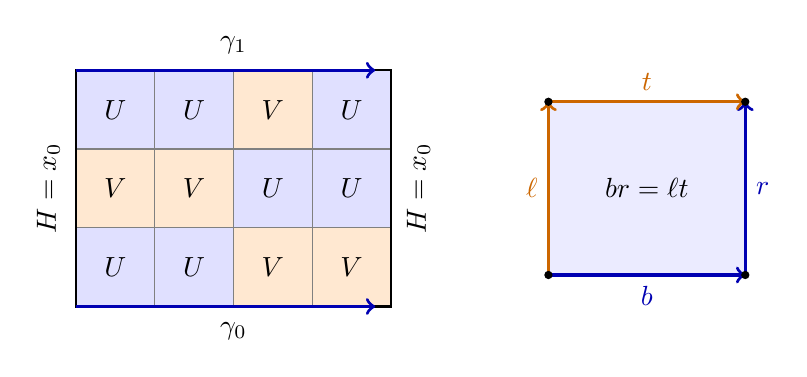
\begin{tikzpicture}[x=1cm,y=1cm]
	\foreach \x/\y in {0/0,1/0,2/1,3/1,0/2,1/2,3/2}{
		\fill[blue!12] (\x,\y) rectangle +(1,1);
	}
	\foreach \x/\y in {2/0,3/0,0/1,1/1,2/2}{
		\fill[orange!18] (\x,\y) rectangle +(1,1);
	}
	\draw[step=1,gray] (0,0) grid (4,3);
	\draw[thick] (0,0) rectangle (4,3);
	\foreach \x/\y/\s in {.5/.5/U,1.5/.5/U,2.5/.5/V,3.5/.5/V,.5/1.5/V,1.5/1.5/V,2.5/1.5/U,3.5/1.5/U,.5/2.5/U,1.5/2.5/U,2.5/2.5/V,3.5/2.5/U}{
		\node at (\x,\y) {\(\s\)};
	}
	\draw[very thick,->,blue!70!black] (0,0)--(3.8,0);
	\draw[very thick,->,blue!70!black] (0,3)--(3.8,3);
	\node[below] at (2,-.08) {\(\gamma_0\)};
	\node[above] at (2,3.08) {\(\gamma_1\)};
	\node[rotate=90] at (-.35,1.5) {\(H=x_0\)};
	\node[rotate=90] at (4.35,1.5) {\(H=x_0\)};
	\fill[blue!8] (6,.4) rectangle (8.5,2.6);
	\draw[very thick,blue!70!black,->] (6,.4)--(8.5,.4) node[midway,below] {\(b\)};
	\draw[very thick,blue!70!black,->] (8.5,.4)--(8.5,2.6) node[midway,right] {\(r\)};
	\draw[very thick,orange!80!black,->] (6,.4)--(6,2.6) node[midway,left] {\(\ell\)};
	\draw[very thick,orange!80!black,->] (6,2.6)--(8.5,2.6) node[midway,above] {\(t\)};
	\node at (7.25,1.5) {\(br=\ell t\)};
	\foreach \x/\y in {6/.4,8.5/.4,6/2.6,8.5/2.6}{
		\fill (\x,\y) circle (1.5pt);
	}
\end{tikzpicture}

	\caption[同伦方格中的道路替换]{同伦方形被细分，使每个小格的像落在一个开集中。右图把一个小格的下边后右边换为左边后上边；所有边通过连接道路接到同一基点，因而得到群等式 \(br=\ell t\)。}
	\label{g1:fig:van-kampen-grid}
\end{figure}

这个证明也给出泛性质。若 \(f_U:\pi_1(U,x_0)\to K\) 与 \(f_V:\pi_1(V,x_0)\to K\) 满足 \(f_Ui_U=f_Vi_V\)，自由积上的延拓会消去所有关系词，故唯一下降为 \(\pi_1(X,x_0)\to K\)。因此计算的关键是两边的群、交集的群和两条包含同态，而不只是三个群的抽象同构类型。

\subsection{多重交集、基点选择与推广范围}
\label{g1:subsec:0502:03}

有限图常需要同时使用好几个开集。下面给出一个条件稍强、却足以直接使用同一网格证明的多开集版本。它允许任意多个开集，但所有开集共用一个基点。

\begin{corollary}[共同基点的多开集版本]\label{g1:cor:many-set-van-kampen}
	设 \(X=\bigcup_{\alpha\in A}U_\alpha\)，每个 \(U_\alpha\) 都开且包含同一点 \(x_0\)，并且任意非空有限个 \(U_\alpha\) 的交集都道路连通。则包含映射诱导同构
	\[
		\pi_1(X,x_0)\cong
		\left(\mathop{*}_{\alpha\in A}\pi_1(U_\alpha,x_0)\right)\big/N,
	\]
	其中 \(N\) 是所有成对交集闭路在两个因子中所给元素之差
	\(i_{\alpha\beta}(\omega)i_{\beta\alpha}(\omega)^{-1}\) 的正规闭包。
\end{corollary}
\begin{proof}
	对一条道路或一个同伦方形，拉回的开覆盖仍有 Lebesgue 数，故只需要有限段或有限个小矩形。段的交点处，在两个标记的交集中选择连接道路；网格顶点处，在所有相邻小矩形标记的交集中选择连接道路，最多涉及四个开集。改变某段标记时，若它的端点还邻接其他标记，就把端点连接道路选在所有这些标记的交集中，所需交集仍是有限交。假设保证上述选择都能完成。

	其余论证逐项与双开集情形相同：连接道路改变所造成的因子在成对交集关系下相消；共同细分比较不同分段；每条公共网格边在其两侧因子中表示同一元素；逐格等式 \(br=\ell t\) 证明同伦不变。由此构造与自然同态互逆的同态，得到同构。开覆盖可以无限，并不要求 \(X\) 紧；用到紧性的只是道路和同伦的参数空间。
\end{proof}

这里要求所有有限交道路连通，是为了能直接在普通四边网格的顶点选择连接道路。更精细的版本只要求成对与三重交道路连通，并把网格错开，使每个顶点至多接触三个标记；本节的应用使用上述已证明的充分条件。一般没有公共基点、或者交集不道路连通时，需要保留多个基点之间的道路信息，不能直接套用同一个商群公式。

最小的警示就是圆周。取 \(U=S^1\setminus\{-1\}\)、\(V=S^1\setminus\{1\}\)，它们都是可缩开弧，交集却有两个道路分支。若忽略交集的道路连通条件，两个平凡群的自由积会错误地给出平凡群；而\cref{g1:thm:circle-fundamental}已经证明圆周的基本群是 \(\mathbb Z\)。从一条开弧走进另一条开弧后再返回，需要知道经过交集的哪一个分支。只有一个基点的交集基本群没有记录这个信息。

改变基点也不是把记号无条件删去。由\cref{g1:prop:basepoint-change}，道路 \(c:x_0\to x_1\) 给出
\[
	\pi_1(X,x_0)\longrightarrow\pi_1(X,x_1),\qquad
	[\gamma]\longmapsto[\bar c*\gamma*c].
\]
若分别给各个开集选了基点，计算包含同态前必须先指定把它们接到公共基点的道路。更改连接道路通常会把相应元素作共轭；这不改变“加入某条闭路的全部共轭作为关系”的正规闭包，却可能改变具体生成元写出的词。因而群的同构类型可以不依赖某些选择，展示的字母与几何闭路之间的对应仍须写清。

还须注意开性。证明中先把参数区间或方形的开覆盖细分；若把空间任意拆成两个闭子集，拉回覆盖不再提供这种细分保证。下面的图和圆盘附着计算都会明确取开邻域，再通过形变收缩把这些邻域化为易算的对象。

\subsection{图、曲面和去点空间的群展示}
\label{g1:subsec:0502:04}

先看只有边而没有面的空间。这里的有限图是把有限多个闭区间的端点附着到有限个顶点所得的商空间，允许一条边两端相同，也允许两顶点之间有多条边；连通指顶点之间可由有限边路连接。有限图带上述商拓扑，等价地可在每条边赋长度 \(1\) 后用最短边路长度定义度量：边内部的小球是区间，顶点的小球是有限条短边段接成的星形，这些正好给出商拓扑的局部开集。图因而是紧 Hausdorff 空间。

一个不含回路的连通子图称为树。若有限连通图中还有回路，删去该回路的一条边的内部不会破坏顶点间的连通；有限次删除以后得到包含所有顶点的树 \(T\)，称为\term[shengchengshu]{生成树}[spanning tree]。树中任意两顶点间恰有一条不重复顶点的边路：存在性来自连通，若有两条不同的简单边路，分岔后第一次重逢就产生回路。有限树若不止一个顶点，任一最长简单边路的两个端点都只有一条邻边，否则可延长或产生回路。逐次删除这种末端边便知，含 \(v\) 个顶点的树有 \(v-1\) 条边。

树还能形变收缩到任一指定顶点。每次选择一个不同于该顶点的末端顶点，将其唯一邻边按区间坐标线性缩到另一端，其他边保持不动；这些映射在共同端点处相容，故由有限闭集粘合连续。有限次组合便给出保持指定顶点不动的收缩。这是下面去掉树状部分时所需的实际同伦。

\begin{proposition}[有限连通图的基本群]\label{g1:prop:graph-fundamental}
	设 \(G\) 是有 \(v\) 个顶点、\(e\) 条边的有限连通图，\(T\) 是一棵生成树，\(x_0\) 是顶点。则
	\[
		\pi_1(G,x_0)\cong F_{e-v+1}.
	\]
	给每条不在 \(T\) 中的边选定方向，从 \(x_0\) 沿树走到该边起点，走过该边，再沿树返回 \(x_0\)，所得闭路给出一组自由生成元。
\end{proposition}
\begin{proof}
	若没有非树边，\(G=T\) 可缩，结论为平凡群 \(F_0\)。否则对每条非树边 \(d\)，令 \(U_d\) 包含整棵树、整条边 \(d\)，以及其他非树边两端参数长度小于 \(1/3\) 的短边段。每个顶点附近的所有短边段都被包括，所以 \(U_d\) 在图中开；这些集合覆盖 \(G\)，并都包含 \(x_0\)。

	把额外短边段各自线性缩到端点，\(U_d\) 形变收缩到 \(T\cup d\)。树中连接 \(d\) 两端的唯一路径与 \(d\) 组成一个圆周；其余边是附着在这个圆周上的有限树枝，依次收缩末端边就把 \(T\cup d\) 收缩到该圆周。若 \(x_0\) 不在圆周上，收缩时它沿树路移到圆周，再用基点变化公式，得到的生成元正是命题中说明的闭路。因此由\cref{g1:thm:circle-fundamental}及形变收缩不改变基本群，\(\pi_1(U_d,x_0)\cong\mathbb Z\)。

	两个或更多不同 \(U_d\) 的交集只含 \(T\) 及各非树边的端点短边段。缩去这些短边段，再收缩树，交集便可缩，且上述收缩保持 \(x_0\) 不动。因此所有有限交道路连通，成对交集基本群平凡。由\cref{g1:cor:many-set-van-kampen}，\(\pi_1(G,x_0)\) 是每条非树边所贡献的 \(\mathbb Z\) 的自由积。非树边数为 \(e-(v-1)\)，结论成立。
\end{proof}

例如两顶点之间的三条边组成的图有基本群 \(F_2\)。选中间一条边为树，另外两条边各给出一个生成元。虽然在纸面图上它围出两个有界区域，这些区域并不属于图本身，所以没有提供把闭路填满的同伦。往图中加入一张面，才会真正增加关系。

\begin{figure}[htbp]
	\centering
	% !TeX root = ../Book1.tex
\begin{tikzpicture}[x=1cm,y=1cm]
	\draw[very thick,blue!70!black] (0,1.5)--(3,1.5) node[midway,below] {\(T\)};
	\draw[thick,->] (0,1.5) to[bend left=55] node[midway,above] {\(d_1\)} (3,1.5);
	\draw[thick,->] (0,1.5) to[bend right=55] node[midway,below] {\(d_2\)} (3,1.5);
	\fill (0,1.5) circle (2pt) node[left] {\(x_0\)};
	\fill (3,1.5) circle (2pt);
	\node[align=center] at (1.5,-.25) {\(e=3,\ v=2\)\\\(\pi_1=F_2\)};
	\fill[blue!8] (5.5,.3) rectangle (7.9,2.7);
	\draw[thick] (5.5,.3) rectangle (7.9,2.7);
	\draw[very thick,blue!70!black,->] (5.9,.3)--(7.5,.3) node[midway,below] {\(a\)};
	\draw[very thick,blue!70!black,->] (5.9,2.7)--(7.5,2.7) node[midway,above] {\(a\)};
	\draw[very thick,orange!80!black,->] (5.5,.7)--(5.5,2.3) node[midway,left] {\(b\)};
	\draw[very thick,orange!80!black,->] (7.9,.7)--(7.9,2.3) node[midway,right] {\(b\)};
	\node[align=center] at (6.7,1.5) {附着圆盘\\\(aba^{-1}b^{-1}=1\)};
	\node at (6.7,-.3) {\(\pi_1(T^2)=\mathbb Z^2\)};
\end{tikzpicture}

	\caption[图的生成元与附着面的关系]{左图中间的蓝边是一棵生成树，其余两边分别贡献自由生成元；纸面上围出的区域不属于图。右图的方形内部则是实际加入的圆盘，按箭头识别对边后，其边界词给出关系 \(aba^{-1}b^{-1}=1\)。}
	\label{g1:fig:graph-and-cell}
\end{figure}

\begin{proposition}[附着一个圆盘]\label{g1:prop:attach-disk}
	设 \(X\) 是道路连通的紧 Hausdorff 空间，\(f:S^1\to X\) 连续，\(x_0=f(1)\)。令
	\[
		Y=X\cup_fD^2=(X\sqcup D^2)/(z\sim f(z)\text{ 对所有 }z\in S^1),
	\]
	即只把圆盘边界按 \(f\) 附着到 \(X\)。记边界闭路为 \(\beta(t)=f(e^{2\pi it})\)。则包含映射给出满同态，且
	\[
		\pi_1(Y,x_0)\cong\pi_1(X,x_0)/\langle\!\langle[\beta]\rangle\!\rangle.
	\]
\end{proposition}
\begin{proof}
	先交代这个商空间及所用收缩的连续性。圆盘内部没有识别，其像是开子空间。对 \(X\) 中的开集 \(O\)，集合
	\[
		O\ \cup\ \{ru:1-\varepsilon<r\le1,\ u\in S^1,\ f(u)\in O\}
	\]
	在商空间中给出 \(O\) 的开邻域；这里边界点已按 \(f\) 识别。若 \(X\) 中两点不同，取不交开邻域 \(O_1,O_2\)，上述邻域也不交。若一个点在圆盘内部，则取半径较大的薄边界环带把它与 \(X\) 分开；两个圆盘内部点用普通小圆盘分开。因此 \(Y\) 为 Hausdorff 空间，且由紧空间 \(X\sqcup D^2\) 的连续像而紧。相同邻域描述也表明 \(X\) 到其像为同胚。

	记圆盘中心的像为 \(o\)，取开集 \(U=Y\setminus\{o\}\) 与 \(V=\{z\in D^2:|z|<2/3\}\) 的像。它们覆盖 \(Y\)，\(V\) 为开圆盘，而交集是 \(0<|z|<2/3\) 的环带。\(U\) 形变收缩到 \(X\)：保持 \(X\) 不动，把每个 \(ru\)（\(r>0\)）送到 \(((1-t)r+t)u\)，终点 \(u\) 按附着关系就是 \(f(u)\)。在边界上公式始终给出 \(f(u)\)，所以与 \(X\) 上的恒等映射相容。为核验同伦一起连续，可注意商映射 \(q:X\sqcup D^2\to Y\) 与 \(\operatorname{id}_{[0,1]}\) 的积是紧空间到 Hausdorff 空间的连续满射，故为闭商映射；限制到开集 \(U\times[0,1]\) 的原像后仍为商映射，上述相容的连续公式遂下降为连续同伦。

	在交集中取基点 \(y_0=1/2\)，其基本群由逆时针圆周 \(t\mapsto\tfrac12e^{2\pi it}\) 生成。径向收缩把这个闭路送到 \(\beta\)；把 \(x_0\) 与 \(y_0\) 沿半径连接并使用基点变化，就得到交集群到 \(\pi_1(U)\) 的像由 \([\beta]\) 生成。另一边 \(V\) 可缩，包含同态把这个生成元送到单位元。由\cref{g1:thm:van-kampen}，商去的正是 \([\beta]\) 的正规闭包。最后沿同一半径把基点换回 \(x_0\)，便得到陈述中的包含同态及其核。
\end{proof}

为何要取正规闭包，而不只删掉整数次的 \(\beta\)？从 \(x_0\) 先沿另一条闭路 \(\eta\) 绕一段，再走圆盘边界，最后沿 \(\bar\eta\) 返回，也能利用同一张圆盘收缩。因此 \([\eta][\beta][\eta]^{-1}\) 必须同时成为单位元。有限次附着圆盘时可逐次应用上面的命题；每一步仍是紧 Hausdorff 空间，最终加入所有附着边界词的关系。

\begin{example}[三个曲面模型的群]\label{g1:exm:surface-presentations}
	环面 \(T^2\) 的基本群为 \(\mathbb Z^2\)，实射影平面 \(\mathbb RP^2\) 的基本群为 \(\mathbb Z/2\mathbb Z\)，从环面去掉一点所得空间的基本群为 \(F_2\)。
\end{example}
\begin{proof}
	在\cref{g1:thm:torus-square}的方形模型中，边界识别后成为有一个顶点、两条环边 \(a,b\) 的图。从左下角出发，逆时针沿方形边界走，依次读出
	\[
		aba^{-1}b^{-1}.
	\]
	方形的内部是一张附着到这个图上的圆盘，故附着命题与图的计算给出
	\[
		\pi_1(T^2)\cong\langle a,b\mid aba^{-1}b^{-1}=1\rangle\cong\mathbb Z^2.
	\]
	这也与\cref{g1:prop:product-fundamental}和 \(T^2=S^1\times S^1\) 的计算相合。边界词记录了具体的附着方向，不是仅凭图形有两个“洞”猜出两个交换的生成元。

	实射影平面可由闭圆盘边界上的对径点识别得到。确切地，将 \(D^2\) 同胚地送到 \(S^2\) 的上半球，再送到对径商 \(S^2/\{\pm1\}\)：每个对径类都有上半球代表，上半球内部的代表唯一，赤道上的两个对径代表恰好被识别。于是得到从圆盘边界对径商到 \(\mathbb RP^2\) 的连续双射；源空间紧，目标由\cref{g1:thm:real-projective-quotient}为 Hausdorff，故是同胚。

	边界自身的商仍是圆周，其坐标可写为 \(e^{i\theta}\mapsto e^{2i\theta}\)。所以绕圆盘边界一周在商圆周上走两周，附着词为 \(a^2\)。得到
	\[
		\pi_1(\mathbb RP^2)\cong\langle a\mid a^2=1\rangle\cong\mathbb Z/2\mathbb Z.
	\]
	最后从环面方形模型的内部去掉中心点，剩下的方形沿从中心发出的射线形变收缩到边界，边界点保持不动，所以同伦与对边识别相容。也可把方形看作圆盘后直接用附着命题证明中的 \(U\) 的径向收缩。所得图是两个圆周在一点相接，故去点环面的基本群为 \(F_2\)。去掉任意其他一点得到相同结论，因为积模型中的旋转 \((z,w)\mapsto(cz,dw)\) 可将任一点移到指定点。
\end{proof}

这些计算针对已经明确构造的曲面，没有使用曲面分类定理。更一般地，若一个多边形模型的边界识别后是一顶点图，先给图中的环边选方向，再沿多边形边界读出词 \(w\)，上述命题便给出 \(\langle a_1,\ldots,a_r\mid w=1\rangle\)。若要断言某个任意给定的曲面必属于某类多边形模型，还需要下一章的分类论证；群展示本身不承担这一任务。

\begin{proposition}[高维球面的单连通性]\label{g1:prop:sphere-simply-connected}
	对每个整数 \(k\ge2\)，球面 \(S^k\) 单连通。
\end{proposition}
\begin{proof}
	当 \(k\ge2\) 时，\(S^k\) 去掉北极或南极得到两个开集，各由球极投影同胚于 \(\mathbb R^k\)：写点为 \((x,t)\in\mathbb R^k\times\mathbb R\)，从北极投影为 \(x/(1-t)\)，逆映射为
	\[
		u\longmapsto\left(\frac{2u}{1+\lVert u\rVert^2},
		\frac{\lVert u\rVert^2-1}{1+\lVert u\rVert^2}\right).
	\]
	南极情形将末坐标变号。这两个开集可缩，交集由
	\[
		(v,t)\longmapsto(\sqrt{1-t^2}\,v,t)
	\]
	同胚于 \(S^{k-1}\times(-1,1)\)，因而道路连通。这里 \(S^{k-1}\) 道路连通可直接看出：两个不对径的单位向量用线段归一化连接，对径时先经一个不与它们共线的单位向量。两个开集道路连通且交集非空，故球面道路连通；再由 van Kampen 定理，两个平凡群的自由积再取商仍平凡，所以 \(\pi_1(S^k)=1\)。
\end{proof}

\begin{proposition}[欧氏空间去掉有限个点]\label{g1:prop:punctured-euclidean}
	设 \(P\subseteq\mathbb R^n\) 是含 \(m\) 个点的有限集合。若 \(n=2\)，则 \(\mathbb R^2\setminus P\) 道路连通，基本群同构于 \(F_m\)，可选从基点出发绕各缺失点一周再返回的闭路作为自由生成元。若 \(n\ge3\)，则 \(\mathbb R^n\setminus P\) 单连通。
\end{proposition}
\begin{proof}
	先说明单点情形。平移把缺失点移到原点，公式
	\[
		H(x,t)=\left(1-t+\frac{t}{\lVert x\rVert}\right)x
	\]
	把 \(\mathbb R^n\setminus\{0\}\) 形变收缩到 \(S^{n-1}\)。当 \(n=2\) 时得到 \(\mathbb Z\)；当 \(n\ge3\) 时，\(n-1\ge2\)，由\cref{g1:prop:sphere-simply-connected}得到单连通性。

	对一般 \(m\) 归纳，\(m=0\) 是可缩的欧氏空间。为使 \(P\) 中各点的第一坐标互不相同，考虑 \(v(t)=(1,t,\ldots,t^{n-1})\)：对任意两不同点之差 \(d\)，内积 \(\langle d,v(t)\rangle\) 是非零多项式，只有有限个实根。取 \(t\) 避开有限个点差所对应的全部实根，再以 \(v(t)\) 的方向为第一坐标轴，就得到所需坐标。取相邻的两个第一坐标之间的数 \(a<b\)，令开条带 \(a<x_1<b\) 不含缺失点，并使 \(x_1<b\) 的开半空间只含最左边的一个缺失点。于是
	\[
		U=(\{x_1<b\}\setminus P),\qquad
		V=(\{x_1>a\}\setminus P)
	\]
	覆盖补空间，交集是凸开条带。每个开半空间同胚于 \(\mathbb R^n\)，例如第一坐标可用 \(\log(b-x_1)\) 或 \(\log(x_1-a)\) 替换，其余坐标不变。因此 \(U\) 是一个点的补空间，\(V\) 对应 \(m-1\) 个点的补空间；它们由归纳假设道路连通，交集可缩。van Kampen 定理给出两基本群的自由积。平面情形为 \(\mathbb Z*F_{m-1}=F_m\)，高维情形为平凡群。

	取交集中的公共基点，并逐次沿条带及半空间中的道路连接到各个小圆周，便得到陈述中的自由生成元；道路的改变会改变所选基及其共轭表达，不改变自由群的同构类型。这个归纳同时证明了补空间道路连通，因为两个道路连通开集有非空交集。
\end{proof}

去点空间说明维数会改变绕行障碍：在平面中，一个缺失点留下一个自由生成元；在至少三维时，闭路可以借额外方向绕过该点并收缩。它也提醒我们不要把“各点绕数都为零”当成平面多点补空间中闭路可收缩的判据，自由群还保留走法的次序。相关的一般方法可参阅\cite[Section 1.2]{Hatcher2002}。
% 纲要条目排为编号小节标题，并进入目录与书签；说明段仍保留于纲要注释中。
